\section{Datenmessung}
 
\subsection{Erkenntnisse aus dem ersten Testlauf}
Nach dem ersten Testlauf mit der Android-App und dem instrumentierten Schüttgut konnten neue wichtige Erkenntnisse gewonnen werden.
Zwischen der App und dem Mikrocontroller kam es zu häufigen Verbindungsabbrüchen. In der App gibt es noch einige Unstimmigkeiten, die behoben werden sollten, damit verwertbare Daten aufgezeichnet werden können: 

\begin{itemize}
	\item Es muss einen fortlaufenden Zähler vom Mikrocontroller geben, damit nach einem Verbindungsabbruch und -wiederaufbau der Zähler mitten im Messlauf weiterläuft und nicht durch eine Zurücksetzung fälschlicherweise eine neue Testrunde  markiert
	\item Beheben eines Bugs beim Datenaufzeichnen nach dem ersten Verbindungsabbruch
	\item Der Zugriff auf die UI-Elemente ist zu hoch. Die Ausgabe auf die UI ist langsamer, als die eingehenden Daten ankommen, weshalb die App ab zu vielen Ausgaben eingefroren ist. Ab dann konnten bisher empfangene Daten auch nicht mehr gespeichert werden
	\item Das Speichern sollte performanter sein
	\item Wie lässt sich ein Rundendurchlauf bzw einzelne markante Punkte in der Anlage währen der Datenaufzeichnung markieren, um nachträglich die analysierten Daten evaluieren zu können?
	\item Bluetooth funktioniert über eine Reichweite zwischen 5-10 Metern. Bei zu vielen Verbindungsabbrüchen muss mit dem Empfangsgeräte an der Anlage mitgelaufen werden, da die Wände der Anlage etwas zu abschirmend sind. Eventuell gibt es eine Möglichkeit mehrere BLE-Empfänger an der Anlage zu positionieren
	\item Zum Schutz des Bauteils wurde die Kapsel in Polsterfolie eingepackt. Dadurch wurde das Bauteil langsamer durch die Anlage befördert als die Steine
	\item Ein Akku mit 100 mAh hält länger als anfangs angenommen
\end{itemize}

\subsection{Erster Messlauf}

Nach Optimierung der Android App konnten wieder Daten gemessen werden. Der Bluetooth-Verbindungsaufbau wurde überarbeitet, sodass die Verbindung nun viel stabiler läuft. Pro Rundendurchgang wurde ein interner Zähler der App auf zurückgesetzt, um Runden im Datensatz identifizieren zu können. Zusätzlich wurde an immer gleichen Punkten der Anlage die empfangen Daten zwischengespeichert: Übergänge von Rüttler auf Förderband und andersrum, Ausnahmen: Langes Förderband auf Querrüttler oben und ganz kurzer Rüttler bis Sortierband. Da damit eine neue Datei angelegt wurde, können auch einzelne Anlagenabschnitte innerhalb eines Messlaufs zugeordnet werden.

Die Kapsel wurde bei den ersten Messrunden in Polsterfolie eingepackt (Abbildung \ref{fig:k4_polsterfolie}). Da dadurch die Kapsel auf der Anlage langsamer als die Steine befördert wurde, wurden an die Verpackung noch drei Flügel, wie in Abbildung \ref{fig:k4_fluegel} zu sehen, angebracht. Dadurch sollen Steine die Kapsel besser mitnehmen können. Damit war die Kapsel ebenso schnell wie die Steine und lag auch auf den einzelnen Beförderungsmodulen sehr stabil, d.h. wenige Orientierungsänderungen. Zum Abschluss wurde die Kapsel ohne Verpackungsmaterial durch die Anlage geschickt (Abbildung \ref{fig:k4_kapsel}). Die Kapsel war hier ebenso schnell wie die Steine. Allerdings war hier zu beobachten, dass die Kapsel sich stark um die Längsachse drehte. 

In den letzten Dateien kam es zu Testfehlern, in der keine aktuellen Daten vom Sensormodul mehr gesendet wurden.

\begin{figure}[htb]
	\centering
	\begin{minipage}[t]{0.49\linewidth}
		\centering
		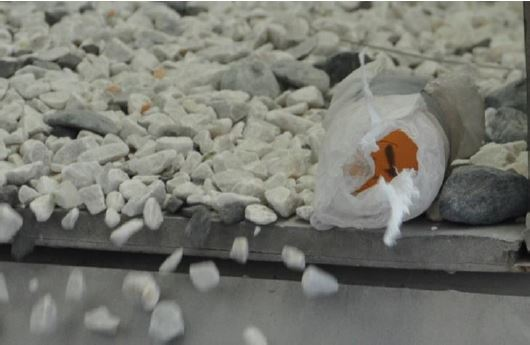
\includegraphics[width=1\linewidth]{images/k4-polsterfolie.JPG}
		\caption{Variante 1: Kapsel in Polsterfolie eingepackt}
		\label{fig:k4_polsterfolie}
	\end{minipage}% <- sonst wird hier ein Leerzeichen eingefügt
	\hfill
	\begin{minipage}[t]{0.49\linewidth}
		\centering
		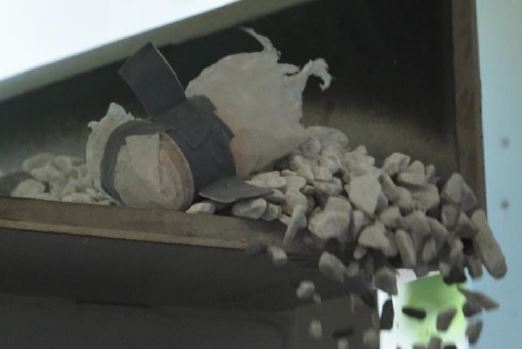
\includegraphics[width=\linewidth]{images/k4-fluegel.JPG}
		\caption{Variante 2: Die Polsterverpackung der Folie wurde mit drei Flügeln aus Duct-Tape erweitert}
		\label{fig:k4_fluegel}
	\end{minipage}
\end{figure}

\begin{figure}[htb]
	\centering
	\begin{minipage}[t]{0.49\linewidth}
		\centering
		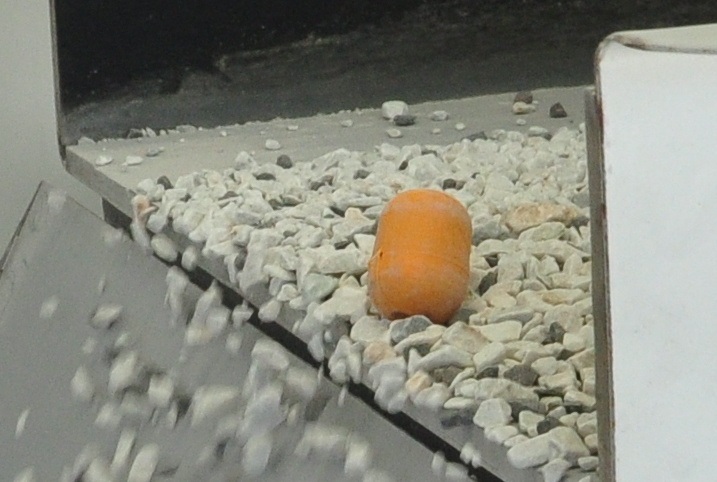
\includegraphics[width=1\linewidth]{images/k4-kapsel.JPG}
		\caption{Variante 3: Die unverpackte Kapsel in der Anlage}
		\label{fig:k4_kapsel}
	\end{minipage}% <- sonst wird hier ein Leerzeichen eingefügt
\end{figure}

\subsection{Zweiter Messlauf}

In einem weiteren Messlauf wurde noch einmal die Auswirkungen der Form des instrumentierten Schüttguts getestet. Dafür wurde wie in Abbildung \ref{fig:k4_alu} und \ref{fig:k4_alurahmen} die Kapsel in einen viereckigen Alu-Rahmen  mit Duct Tape fixiert. Damit kann das Verhalten eines Schüttguts mit rechteckiger Form getestet werden. 

\begin{figure}[htb]
	\centering
	\begin{minipage}[t]{0.49\linewidth}
		\centering
		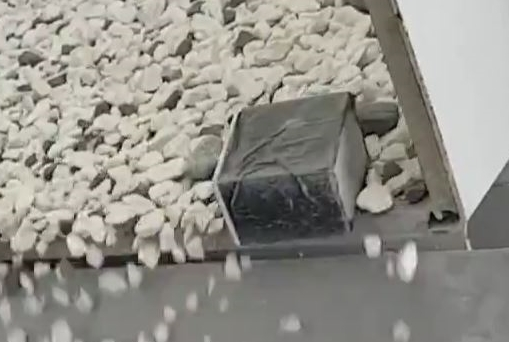
\includegraphics[width=\linewidth]{images/k4-alu.JPG}
		\caption{Variante 4: Die Kapsel ist in einen Alurahmen geklebt, um eine Kastenform zu erhalten}
		\label{fig:k4_alu}
	\end{minipage}% <- sonst wird hier ein Leerzeichen eingefügt
	\hfill
	\begin{minipage}[t]{0.49\linewidth}
		\centering
		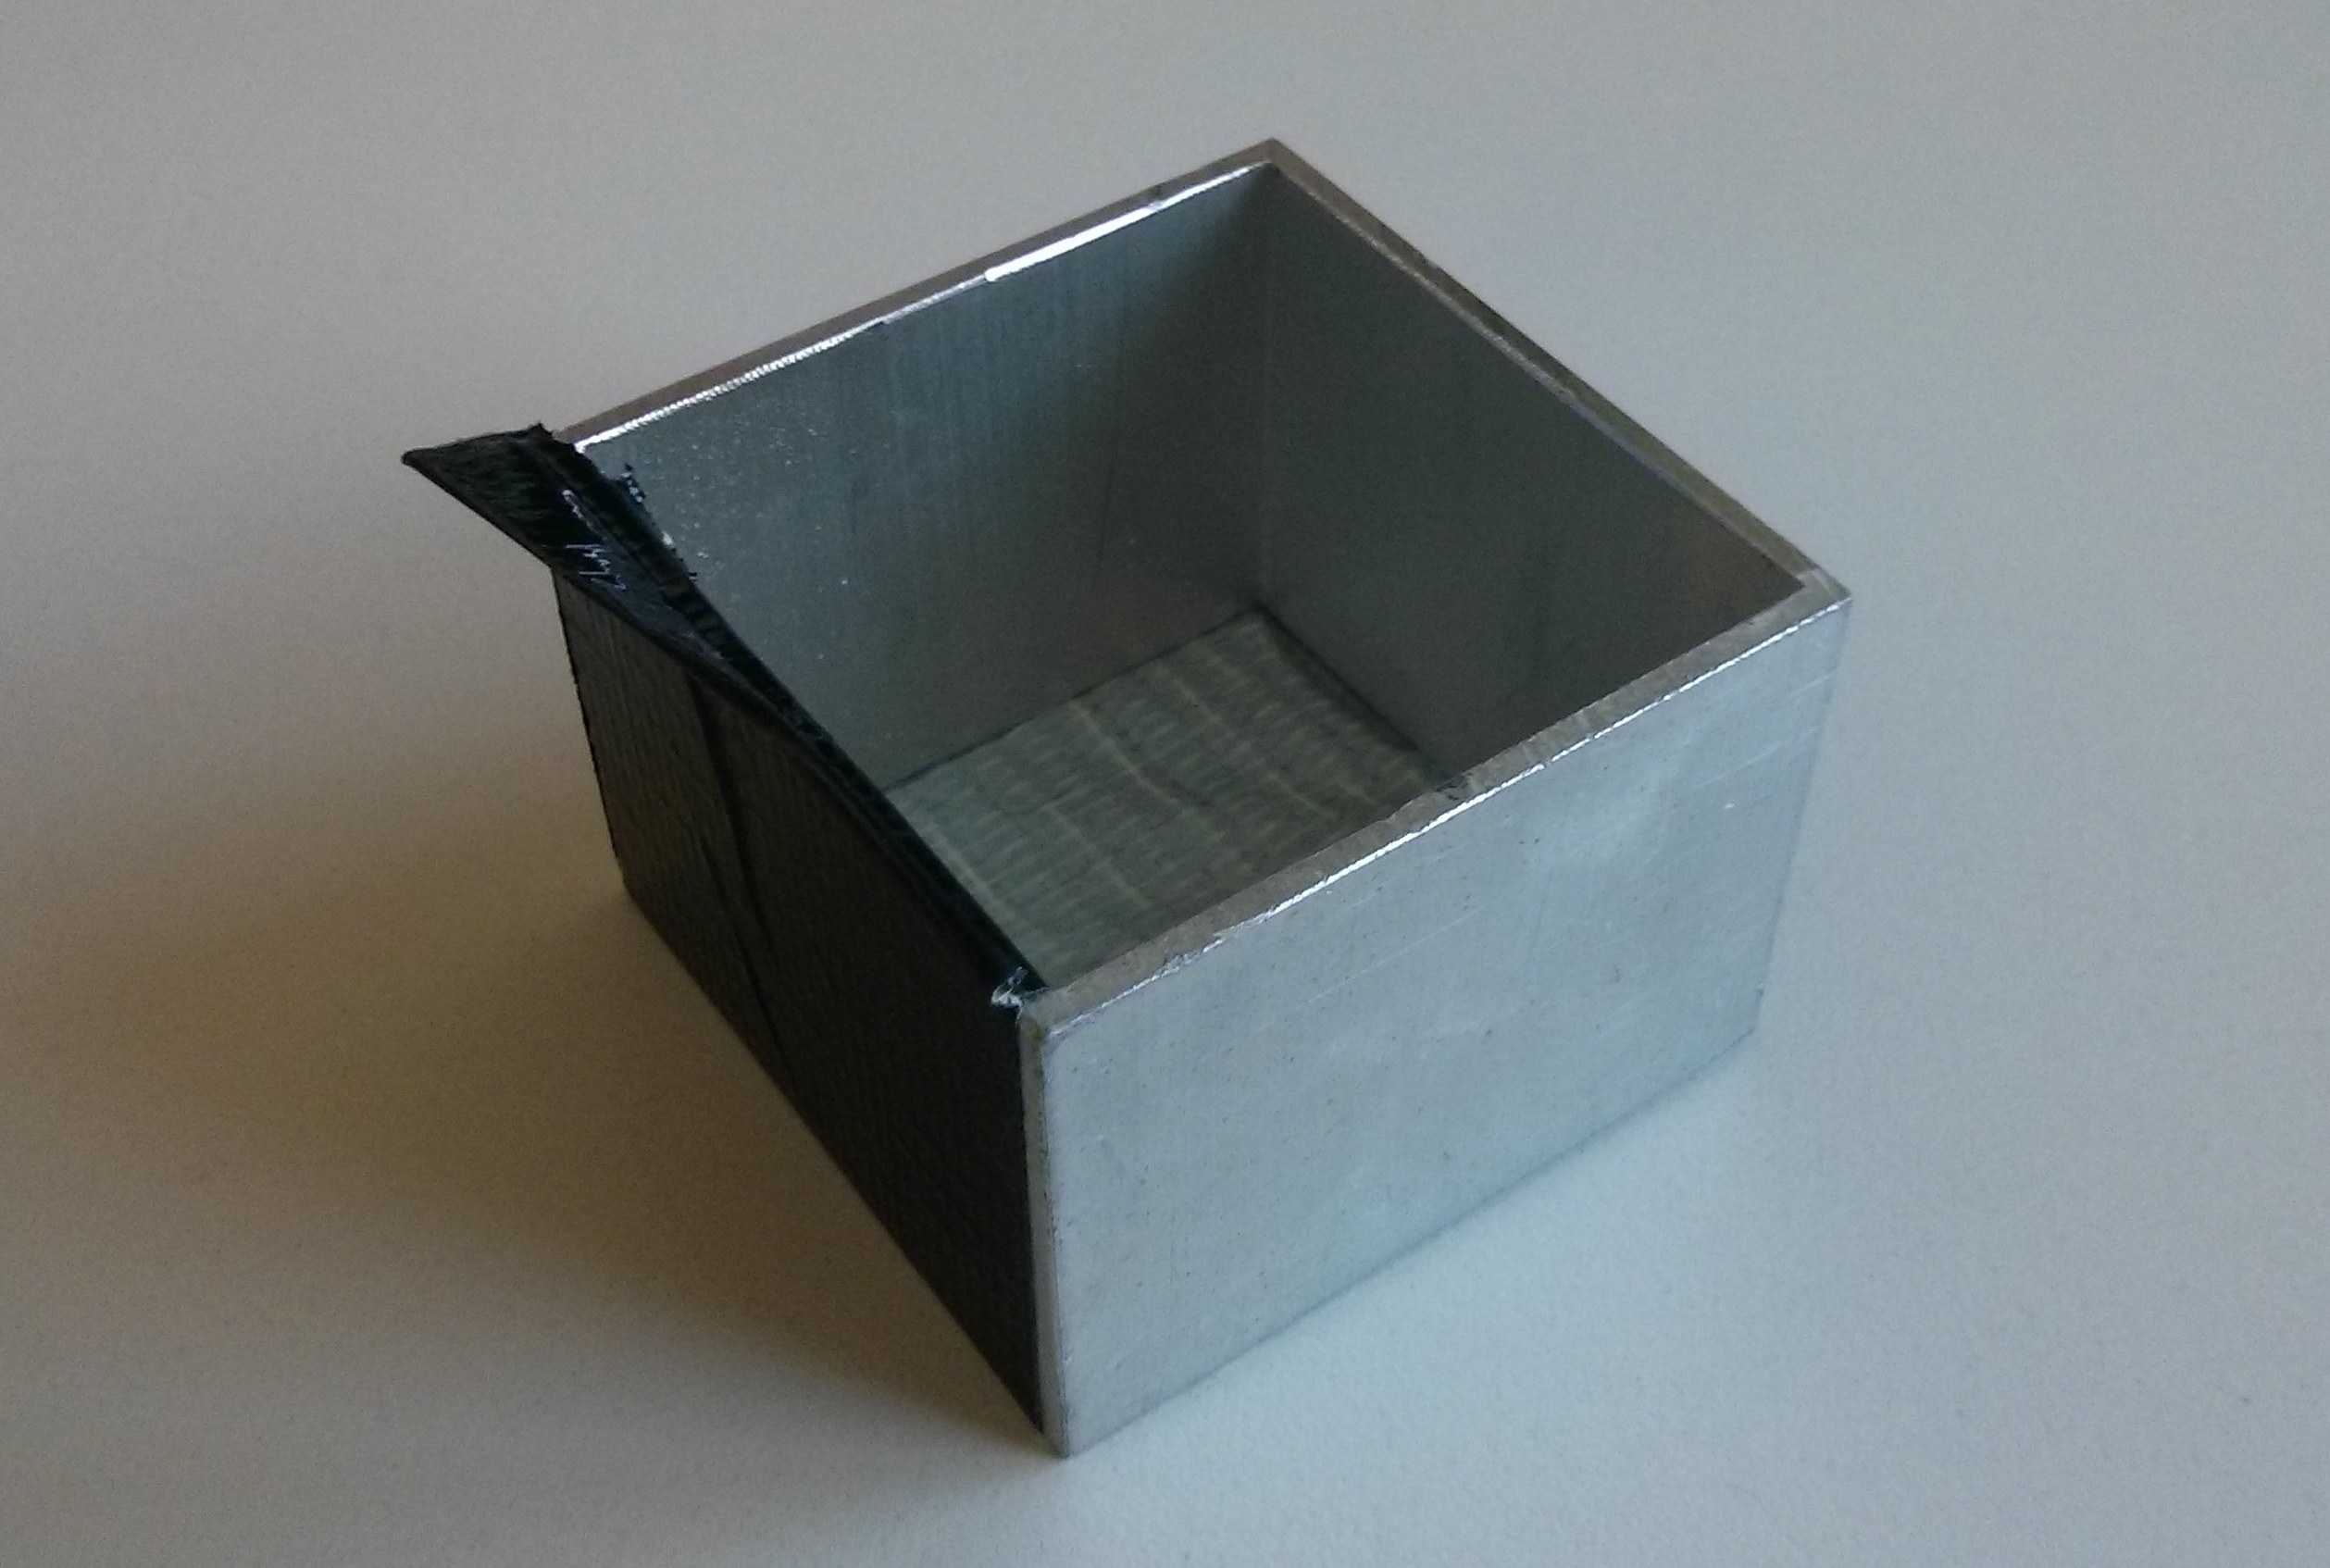
\includegraphics[width=\linewidth]{images/k4-alurahmen.jpg}
		\caption{Variante 4: Die Kapsel wird mittels Duct Tape im Alurahmen fixiert}
		\label{fig:k4_alurahmen}
	\end{minipage}
\end{figure}

Nach fünf Testrunden und der Kontrolle der gespeicherten Datendateien musste leider festgestellt werden, dass vom Mikrocontroller fehlerhafte Sensorwerte geliefert wurden. Beim Ausweichen auf ein anderes instrumentietes Schüttgut musste zunächst ein Kabel verlötet werden, das abgebrochen war. Dies zeigt, dass die Mikrocontroller nicht sehr robust sind, allerdings auf der Anlage auch starken Vibrationen und Erschütterungen ausgesetzt sind.

Nach einem Verbindungsaufbau mit der Android App war jedoch ein fehlerfreies Empfangen der Daten mit dem weiteren Mikrocontroller nicht möglich. Es kamen geringer getaktete Datentupels an, begleitet von vielen Bluetooth-Verbindungsabbrüchen. Eventuell beeinträchtigt ein Alurahmen die Bluetooth-Verbindung, weswegen man zukünftig auch noch weitere Materialien testen sollte. Widersprüchlich ist nur, dass der erste Mikrocontroller trotz des Rahmens senden konnte. Daraus ergibt sich auch die Notwendigkeit, vor Messbeginn Referenzmessungen mit jedem verwendeten instrumentierten Schüttgut durchzuführen, um festzustellen, ob es unterschiedliche Verhalten bei den einzelnen Adafruit-Bauteilen gibt.

Obwohl keine gemessenen Sensordaten zur Verfügung stehen, konnte beobachtet werden, dass der Alurahmen auf den Förderbändern sehr ruhig liegend befördert wurde. Auf den Rüttlermodulen jedoch drehte sich die Box auch und sprang teilweise sogar einige Zentimeter zurück. Auch das Oberflächenmaterial könnte eine wichtige Rolle spielen. Sowohl Variante 3 mit der unverpackten Kapsel und Variante 4 mit Duct Tape und Alurahmen haben eine sehr glatte Oberfläche, bei denen auch ein unruhiges Laufverhalten beobachtet werden konnte.
